\capitulo{4}{Técnicas y herramientas}

Esta sección presenta un breve resumen de las técnicas y herramientas que han sido usadas para llevar a cabo este trabajo.

\section{Técnicas}

\subsection{Modelo-Vista-Controlador}
Se ha hecho uso del patrón MVC para el desarrollo del proyecto. Este patrón permite la separación de la lógica de negocio de los datos y las vistas. Como su nombre indica, sus componentes quedan divididos en:

\begin{itemize}
	\item \textbf{Modelo:} representa los datos y la lógica de negocio.
	\item \textbf{Vista:} presenta la información del modelo.
	\item \textbf{Controlador:} controla las entradas del usuario y selecciona la vista.
\end{itemize}

\begin{figure}[h]
  \centering
    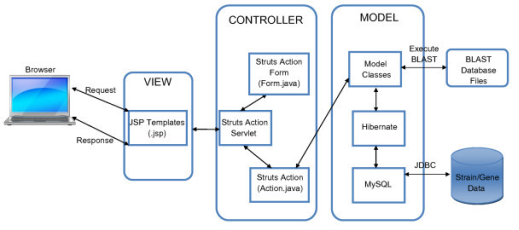
\includegraphics[width=0.6\textwidth]{../img/diagramas/mvc.png}
  \caption{Modelo-Vista-Controlador.}
  \label{ciclo}
\end{figure}

En el Anexo referente al Manual de Programación se detalla la estructura del proyecto según este patrón.

\subsection{Diseño Web Centrado en el Usuario}

A la hora de realizar una página web es fundamental tener en cuenta al usuario final de la misma, por tanto, siempre se ha de tener presente que la calidad de diseño es algo fundamental. El diseño de la plataforma modelará la interacción entre el usuario y la aplicación. De esta forma, un buen diseño, facilitará la consecución de los objetivos del usuario, mientras que un diseño pobre hará que el usuario busque otro medio por el que conseguir sus objetivos.

Durante el desarrollo de este proyecto se ha tenido siempre en cuenta el Diseño Centrado en el Usuario. En este apartado se darán algunas nociones sobre este aspecto tan importante a la hora de que un sitio web sea accesible y usable por todo tipo de usuarios.

En esta sección se va a tratar el diseño centrado en el usuario, siguiendo el trabajo presentado en el trabajo realizado por Yusef Hassan-Montero, Francisco J. Martín Fernández y Ghzala Iazza.


\subsubsection{Usabilidad y accesibilidad}

La usabilidad es un anglicismo que quiere decir que algo es de fácil uso. Aunque hay multitud de definiciones, se puede dar la ofrecida por la Organización Internacional de Estandarización (ISO). La ISO define usabilidad como: \quotes{Grado de eficacia, eficiencia y satisfacción con la que usuarios específicos pueden lograr objetivos específicos en contextos de uso específicos}. Mediante esta definición se pueden apreciar dos tipos de atributos diferenciados.

\begin{itemize}
	\item Atributos cuantificables de forma objetiva: como pueden ser la eficacia o el número de errores
		que comete un usuario al realizar una tarea y la eficiencia o tiempo que ha necesitado el usuario para llevar a cabo una tarea en concreto.
	\item Atributos cuantificables de forma subjetiva: como puede ser la satisfacción de uso de la
plataforma web por parte de un usuario concreto.
\end{itemize}

Aunque no siempre se va a poder dotar a la aplicación o plataforma de una usabilidad universal, es decir, que sea usable para todos los posibles tipos de usuarios, a la hora de diseñar dicha plataforma, se ha de tener en cuenta quiénes serán los usuarios potenciales y qué necesidades y conocimientos tienen.

Otro concepto ligado de forma íntima a la usabilidad es la accesibilidad. Esto es, el diseño ha de posibilitar el acceso a la información a la mayor cantidad de usuarios posibles. No sólo consiste en facilitar el acceso a personas invidentes, sino que también se ha de prever el acceso desde conexiones lentas, hardware y software no actualizados, etc. En este punto se puede observar una contradicción ya que un diseño usable puede que deba centrarse en un tipo de usuario en concreto, mientras que la accesibilidad trata de universalizar la posibilidad de acceso de los usuarios al sitio web.

En este proyecto se hace especial énfasis en la usabilidad del sitio, haciendo que los menús y
opciones sean lo más sencillos y claros posibles.

\subsubsection{Arquitectura de información}

Aunque un usuario típico pensará que la interfaz es la aplicación puesto que es la parte de dicha aplicación con la que interactúa, se debe entender que la usabilidad de una aplicación depende en gran medida de su arquitectura, es decir, depende del componente no visible del diseño. Por este motivo, es importante una elaboración óptima del backend (lógica de la aplicación) para que el uso del portal web sea lo más sencillo e intuitivo posible.

La Arquitectura de la Información (AI) se puede definir como \quotes{el arte y la ciencia de organizar espacios de información con el fin de ayudar a los usuarios a satisfacer sus necesidades de información}. La actividad de organizar la información, incluye la estructuración, la clasificación y el rotulado de los contenidos de la aplicación.

\subsubsection{Recuperación de la información}

El principal objetivo de un correcto diseño de la AI es que permita al usuario recuperar la información de la forma más sencilla posible. El objetivo de este portal web es permitir al usuario analizar rutas y visualizar los resultados sobre mapas permitiendo ver toda la información disponible mediante el uso de dichos mapas y tablas. De esta forma, un usuario en concreto, podrá comprender de mejor forma los datos obtenidos de un determinado análisis.


\subsubsection{Visibilidad}

El punto anterior está estrechamente ligado con la visibilidad de la información, es decir, que cada elemento de información pueda ser encontrado. Un usuario que acceda a este portal web, encontrará varias opciones en el menú principal de la aplicación como: \quotes{Tratamiento de ficheros}, \quotes{Visualización de resultados} o \quotes{Gestión}. Quedando
claro el tipo de información que se encontrará en cada página visitada. Si el usuario accede a la página de tratamiento de ficheros, encontrará diversas opciones de gestión de los mismos. Por su parte, si accede a la página de visualización de resultados, podrá encontrar dos secciones diferenciadas. En la primera sección (parte izquierda de la pantalla) podrá elegir el área o áreas sobre las que filtrar las rutas y en la segunda (parte derecha) las rutas encontrada que cumplan con los criterios indicados.

\subsubsection{Diseño web centrado en el usuario}

Para poder afirmar que una aplicación cumple con los niveles de usabilidad requeridos, el diseñador necesita de una serie de técnicas, métodos y procedimientos diseñados para tal fin.

Como se ha comentado desde el comienzo de esta memoria, el trabajo se ha centrado siempre en el usuario, siguiendo la metodología conocida como Diseño Centrado en el Usuario (User-Centered Design) adaptándose a las necesidades y características de una plataforma web.

El Diseño Web Centrado en el Usuario se caracteriza por asumir que todo el proceso de diseño y desarrollo de la plataforma ha de estar conducido por el usuario final y las necesidades y objetivos del mismo.

Centrar el diseño en el usuario, implica involucrar al mismo desde el comienzo. Se ha de conocer al usuario, lo que necesita, cuál será el uso que den a la aplicación, cómo es la experiencia de uso de la misma, etc.

El DiseñoWeb Centrado en el Usuario, usado en este proyecto, se divide en varios pasos o etapas. Como se ve en la Figura \ref{ciclo}, las fases de diseño, prototipado y evaluación son cíclicas. Quiere decir que cada diseño deberá ser evaluado de forma constante. 

\begin{figure}[h]
  \centering
    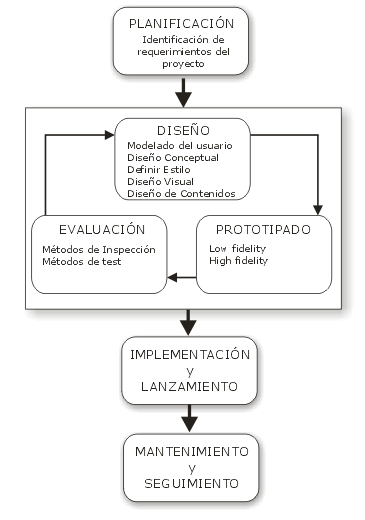
\includegraphics[width=0.6\textwidth]{../img/dwcu/ciclo.png}
  \caption{Esquema del diseño web centrado en el usuario.}
  \label{ciclo}
\end{figure}


A continuación, se procede a explicar cada una de las fases del Diseño Web Centrado en el
Usuario.

\paragraph{Planificación:} En este momento se han de identificar todos los objetivos, necesidades y requerimientos de la plataforma web. Se trata de encontrar un equilibrio entre las necesidades del usuario y lo que un programador puede ofrecer. En este sentido no suele ser fácil obtener toda la información necesaria por parte del usuario. Será importante estudiar a los usuarios potenciales para que el sitio se adapte de la mejor forma posible a sus necesidades.

La etapa de planificación, se basará por tanto, en la recogida de toda la información (lo más detallada posible) con el objetivo de poseer una base sólida sobre la que poder tomar decisiones en las siguientes etapas.

\paragraph{Diseño:} En esta etapa, se tomarán todas las decisiones de diseño en base a la información obtenida en el paso anterior. La fase de diseño se puede dividir en los siguientes puntos:

\begin{itemize}
	\item \textbf{Modelado del usuario:} se tratará de conocer las necesidades de los potenciales usuarios de
la aplicación.
	\item \textbf{Diseño conceptual:} tratará sobre el diseño de contenidos del portal web.
	\item \textbf{Definir el estilo:} se definirá el estilo de todo el sitio web.
	\item \textbf{Diseño visual:} trata de definir el número de colores que serán usados, el tipo de letra, etc.
	\item \textbf{Diseño de contenidos:} en este punto se valorará el contenido que cada sección mostrará al usuario.
\end{itemize}

\paragraph{Prototipado:} Uno de los mayores problemas a la hora de evaluar la usabilidad del sitio web, es que todavía no se encuentra  implementado. La solución, pasa por el uso de prototipos, es decir, modelos de la interfaz de la página, que ayudarán a comprobar la usabilidad. Este prototipado puede ser clasificado en:

\begin{itemize}
	\item \textbf{Prototipado horizontal:} reproducen el aspecto visual del sitio, pero no tienen por qué representar la funcionalidad del mismo.
	\item \textbf{Prototipado vertical:} se reproduce sólo una parte del diseño del sitio, pero además incluye toda la funcionalidad final del mismo.
	\item \textbf{Prototipado de alta fidelidad:} este prototipo será idéntico al sitio web ya terminado.
	\item \textbf{Prototipado de baja fidelidad:} este prototipo podrá ser muy distinto del diseño del sitio web una vez finalizado.
\end{itemize}

Para ahorrar costes y agilizar los primeros pasos, es posible que los primeros diseños estén realizados en papel.

\paragraph{Evaluación:} Existen numerosos métodos para comprobar la usabilidad del sitio web, además de poder ser realizada sobre distintas representaciones de la aplicación.

\paragraph{Implementación y lanzamiento:} Lo más recomendable a la hora de desarrollar un sitio web, es el uso de estándares, como pueden ser, HTML 5 o CSS 3. Así se asegura una compatibilidad y escalabilidad futura. Otro aspecto importante, es que la hoja de estilos (CSS) esté separada del propio contenido HTML del sitio.

En esta etapa es fundamental supervisar que todo funcione como se había especificado, si algo no funciona, no será usable.

En el momento en el que el sitio está acabado y su funcionalidad testada, es posible ponerlo en producción y presentarlo al usuario. Si se cree conveniente es posible diseñar una serie de páginas de ayuda al usuario novel, que le guíen y ayuden en los primeros pasos sobre el sitio web.

\paragraph{Mantenimiento y seguimiento:} Una plataforma web está en constante desarrollo, sus contenidos y audiencia pueden cambiar con el tiempo, el diseño puede cambiar.

Pero es fundamental que ese diseño no varíe de forma drástica de un día para otro siendo estos cambios muy sutiles.

\subsection{Seguimiento de la usabilidad de la plataforma web}

Por último, cabe destacar, que no todos los problemas pueden haber sido descubiertos en las etapas previas. Es importante obtener un feedback (mediante formularios o contacto con el usuario) de la experiencia que el usuario tiene con la web.

\section{Herramientas}
Las herramientas usadas durante la implementación del proyecto se muestran en los siguientes apartados de esta sección.

\subsection{NetBeans}
El IDE elegido para el desarrollo del trabajo ha sido NetBeans en su última versión disponible a la hora de finalizar este proyecto(8.2).

Este entorno ha sido elegido principalmente por haber sido usado en proyectos anteriores y poseer un conocimiento más avanzado del mismo que de otros entornos como puede ser Eclipse.

Atom ha sido usado como editor secundario para manejo de ficheros csv entre otros.

\subsection{Glassfish}
Para desplegar la aplicación web se cuenta con un servidor Glassfih en su versión 4.1.

\subsection{Open Street Maps}
Open Street Maps (OSM) es un proyecto colaborativo que permite crear y editar mapas. Estos mapas son de uso libre y gratuito para todos los usuarios, siendo solo los usuarios registrados los que pueden crear dichos mapas.

La creación de los mapas se lleva a cabo mediante la recogida de coordenadas geográficas usando dispositivos móviles. Estos dispositivos móviles obtendrán su ubicación gracias a sistemas GPS o Glonass o al uso de wifi o a la ubicación proporcionada por el operador de telefonía en caso de que el dispositivo cuente con una tarjeta SIM.

Los mapas son distribuidos bajo licencia ODbL (Licencia Abierta de Bases de Datos).

Los datos se almacenan siguiendo el datum WGS84 (World Geodetic System 1984, constituido por parejas latitud-longitud) usando la proyección de Mercator (definida en 1569  por Gerardus Mercator). La información primitiva consta de:

\begin{itemize}
	\item Nodos: son posiciones geográficas concretas.
	\item Vías: una lista ordenada de nodos constituye una vía. Esta puede ser una polilínea o un polígono.
	\item Relaciones: son grupos de vías, nodos y relaciones que pueden ser agrupadas ya que contienen propiedades comunes.
	\item Etiquetas: son usadas para almacenar metadatos sobre los objetos del mapa, constan de una pareja clave-valor. 
\end{itemize}

\subsection{PostgreSQL 9.6}
PostgreSQL es un Sistema Gestor de Bases de Datos (SGBD) relacional, orientado a objetos y libre, distribuído bajo licencia PostgreSQL License. Actualmente se encuentra en su versión 9.6 siendo la usada en este trabajo.

\subsection{PostGIS}
PostGIS es una Base de Datos espacial que expande las posibilidades de PostgreSQL añadiendo soporte a objetos geográficos permitiendo consultas de localización. PostGIS ha sido diseñado y desarrollado por la empresa Refraction Research siendo distribuido bajo licencia GNU (GPLv2).

\subsection{QGIS}
Para los pasos previos de este trabajo se ha hecho uso del programa QGIS. QGIS es un sistema de información geográfico libre y de código abeirto. Cuenta con una infinidad de opciones, algunas de las más relevantes son:

\begin{itemize}
	\item Conexión con PostgreSQL: permite mantener una conexión contra la Base de Datos que contiene los datos relativos a los análisis de las rutas. De esta forma es posible pintar sobre un mapa todos y cada uno de los puntos de cada ruta analizada. Es posible adaptar las consultas SQL para obtener la información deseada antes de ser pintada.
	\item Uso de diferentes APIs de mapas: permite usar mapas de Open Street Maps, Google Maps, etc.
	\item Descarga de datos OSM: permite la descarga de datos en formato osm indicando el área deseado.
\end{itemize}

\subsection{Osmosis}
Osmosis es una herramienta desarrollada en Java y que funciona por línea de comandos. Permite procesar ficheros OSM con un gran rendimiento debido a que está diseñada para tratar con ficheros de extensión considerable (un fichero osm conteniendo información completa de un país puede superar los 10 GiB de datos).

Esta herramienta permite desde cargar datos sobre una Base de Datos hasta extraer un subconjunto de ellos a partir de un fichero de tipo osm. Además, Osmosis puede formar parte de otras aplicaciones Java incluyéndose como una librería.

\subsection{Osmconvert}
Esta herramienta permite realizar distintas conversiones entre ficheros de distinta extensión. En el caso de este proyecto, la herramienta permite al usuario transformar ficheros de extensión pbf a ficheros osm con los que trabajar posteriormente.

Aunque es muy sencilla de usar, se facilita un script preparado para extraer ficheros pbf.

\subsection{Osmfilter}
Como su nombre indica, la herramienta Osmfilter permite filtrar ficheros osm mediante sus etiquetas. En este trabajo ha sido usada para extraer ficheros de tipo XML a partir de ficheros de extensión osm manteniendo únicamente los Puntos De Interés del área englobada en el fichero original.

Además, se provee al usuario de un sencillo script para hacer uso de esta herramienta a la hora de incluir nuevos Puntos De Interés sobre el sistema.

\subsection{\LaTeX}
Se ha usado \LaTeX  para la relaización de la documentación del presente Trabajo de Fin de Máster. El contenido ha sido editado con TexMaker en su versión 4.5.

\subsection{Lenguajes de programación, marcado y/o SQL}

\subsubsection{HTML 5}
HyperText Markup Lenguage 5 es la última versión del estándar HTML publicado a finales del año 2014 siendo sucesor de la versión 4.01. Incluye nuevas etiquetas dejando otras obsoletas. Es un lenguaje de marcado destinado al desarrollo de páginas web. Es un lenguaje estándar que cualquier navegador web será capaz de reconocer e interpretar.

\subsubsection{Java}
Java es un lenguaje de programación orientado a objeto concurrente y de propósito general. Java mantiene un número de dependencias reducido para permitir la ejecución del programa desarrollado en el mayor número de dispositivos posibles sin ser recompilado.

La primera revisión de este lenguaje fue desarrollada por James Gosling en la ya desaparecida Sun Microsystems (actualmente absorbida por Oracle), siendo cada aplicación Java compilada y ejecutada por una máquina virtual Java (JVM).

Aunque este lenguaje apareció en 1995, no fue hasta 2012 cuando se convirtió en uno de los lenguajes más usados, especialmente en aplicaciones cliente-servidor. La versión estable actual es la 8.

\subsubsection{Servlet}

Un servlet es un componente ubicado en el servidor Java EE encargado de dar respuesta a las peticiones de los clientes. Cada servlet amplía las capacidades del servidor en el que se encuentra pudiendo generar contenido dinámico como pueden hacer PHP o ASP.NET.

El ciclo de vida de un servlet es el siguiente:

\begin{itemize}
	\item Inicialización: el proceso de inicialización (llamada al método init) ha de hacerse antes de que el servlet pueda interaccionar con los clientes.
	\item Interacción: una vez inicializado, el servlet, puede atender a las peticiones de los clientes.
	\item Destrucción: para destruir un servlet se ha de llamar a su método destroy. Este método será llamado cuando el servidor sea cerrado o el administrador del sistema lo requiera. Para inicializar el servlet destruido se ha de llamar al método init de nuevo.
\end{itemize}

\subsubsection{JSP}
Java Server Pages o JSP es una tecnología de vistas que corre en el lado del servidor permitiendo escribir plantillas en lenguajes como HTML, JavaScript o CSS. Una página JSP puede contener segmentos de código implementados en Java que permitan modelar dicha página de forma dinámica.

Una de las ventajas de JSP es su base en Java, permitiendo crear clases de acceso a datos (DAO), lógica de negocio, etc.

Una página JSP permite sintaxis como la siguiente:

\begin{itemize}
	\item Directivas: permiten incluir otros ficheros, clases Java para el manejo de objetos, etc.
	\item Declaraciones: permiten declarar variables, funciones y datos estáticos.
	\item Expresiones: permiten evaluar expresiones Java.
	\item Etiquetas: simplifican el código aportando funcionalidad añadida. Existen dos grandes grupos de etiquetas: las que proporcionan funcionalidad a la página (como jsp:include) y las que permiten manipular componentes JavaBean (como jsp:useBean).
	
\end{itemize}

\subsubsection{CSS 3}
Cascading Style Sheet (CSS) es un lenguaje usado para definir la presentación visual de un documento escrito en HTML y  permitiendo separar la estructura de un documento de su presentación. El estilo puede ser incorporado \quotes{en línea}, mediante una hoja interna o mediante el uso de una hoja de estilo externa.

El principal problema que persiste con el paso de las versiones es el centrado vertical ya que no es sencillo y requiere de más reglas que el centrado horizontal (siendo este último casi automático).

\subsubsection{Bootstrap 3}

Esta plataforma web se ha diseñado pensando en el usuario final de la misma, por tanto, se han tenido en cuenta las pautas marcadas por un diseño adaptable (Responsive Web Design). Este objetivo ha sido posible gracias al uso de un framework como Bootstrap. Este framework permite diseñar el sitio para todos los tamaños de pantalla actuales.

Bootstrap implementa CSS para una gran cantidad de clases, lo que hará que el diseño de la plataforma web sea más sencillo. Unas de las clases más importantes son las que permiten adaptar el contenido mostrado al tamaño de pantalla desde la que la web ha sido accedida.

En Bootstrap el contenido se agrupa en filas (row) y en columnas (col) hasta un máximo de 12 columnas. Por tanto, en las líneas superiores, se crea una fila (row) y el div interno especifica las columnas para un tamaño de pantalla xs o md (estos tamaños ya están predefinidos en Bootstrap). De esta forma tan sencilla se puede agrupar el contenido de ese \quotes{div} mediante el CSS que ya contiene el framework. 

Bootstrap también contiene gran cantidad de estilos para menús, botones, listas, además de colores recibiendo el nombre de componentes. Se pueden encontrar iconos que se podrán usar en botones, en texto, menús de usuario simples o con accesos desplegables, mensajes de alerta con colores llamativos para el usuario, barras de progreso, etc.

\subsubsection{JavaScript y jQuery}

JavaScript (JS) es un lenguaje interpretado, débilmente tipado y dinámico, que cumple el estándar ECMAScript siendo la última versión estable la ECMAScript 2016. En el desarrollo de una página web, se usará en el lado del cliente, permitiendo la generación de páginas dinámicas o la mejora de la interfaz de usuario. En la actualidad, la gran mayoría de los navegadores son capaces de interpretar este lenguaje. JavaScript está provisto de una implementación del DOM (Document Object Model) para poder interactuar con la página web.

Aunque se pueda pensar que Java y JavaScript están relacionados, en realidad, no es así. Inicialmente JavaScript fue diseñado con una sintaxis similar a C aunque adoptando nombres y convenciones similares a las de Java.

jQuery es una biblioteca de JavaScript (presentada en enero de 2006) que pretende simplificar la interacción con los documentos HTML, la manipulación del DOM o el manejo de eventos. Además de permitir una interacción con la técnica AJAX.
En la misma web que la usada para JavaScript se pueden encontrar gran variedad de ejemplos y referencias para el uso de jQuery

En jQuery, se usa la función \$ para interaccionar con las páginas HTML. Recibe como parámetro el nombre de una etiqueta HTML o una expresión en CSS, devolviendo todos los nodos del DOM que concuerdan con esa expresión. Si queremos que esto funcione en Drupal, tenemos que dar un paso más, y es que debemos englobar esta función dentro de otra.

\subsubsection{AJAX}
Asynchronous JavaScript And XML, conocida como AJAX, es una técnica de desarrollo web que permite la implementación de aplicaciones interactivas. Las aplicaciones se ejecutarán en el navegador del cliente y, por detrás, se mantiene una comunicación asíncrona con el servidor. Así, es posible, que la página sea actualizada sin necesidad de realizar una recarga completa de la misma. Con AJAX, se mejora la interactividad, velocidad y usabilidad de estas aplicaciones. AJAX no es una tecnología en sí sino un término que engloba a un conjunto de las mismas que trabajan de forma conjunta. HTML y CSS: para la presentación de la información. Document Object Model (DOM): para mostrar la información e interaccionar con la misma. JSON: para intercambiar datos. XMLHttpRequest: para poder mantener una comunicación asíncrona. JavaScript: para unir estas tecnologías. En la siguiente página web podemos encontrar mucha información relativa tanto a JavaScript como a AJAX en particular.

\subsection{Máquina virtual y sistema operativo}
Se ha optado por instalar el Sistema Operativo Ubuntu 16.04 LTS en una máquina virtual bajo el entorno de Virtual Box. De esta forma, se permite exportar e importar la máquina pudiendo ser instalada en cualquier ordenador. Además, este planteamiento permite hacer uso de la plataforma web de forma offline y sin tener que estar disponible en un servidor.

Además se ha hecho uso de diversos navegadores web como son Chrome, Firefox o Konqueror, para poder comprobar el correcto funcionamiento del sitio, además de la correcta visualización del contenido de la hoja de estilo. Es un punto importante ya que algunos navegadores, en versiones antiguas, puede que no soporten todas las etiquetas del estándar HTML5 o todo los correspondientes estilos de CSS3.
